% =====================================================================
% scidata-sr4all-frame.tex  —  root document (compile this one)
% Scientific Data (Data Descriptor) — no journal template by design.
% =====================================================================
\documentclass[11pt]{article}

% --- Encoding & fonts (Computer Modern, as Sci Data recommends) ---
\usepackage[utf8]{inputenc}
\usepackage[T1]{fontenc}

% --- Core ---
\usepackage{graphicx}
\graphicspath{{figures/}}
\usepackage{booktabs}
\usepackage{siunitx}        % numeric columns in the overview table
\usepackage{amsmath}
\usepackage{fontawesome5}   % \faLink
\usepackage{url}
\usepackage{microtype}


% --- Tables ---
\usepackage{threeparttable}
\usepackage{rotating}       % sidewaystable for the wide overview table

% --- Links: hyperref gives \href for EXTERNAL urls only.
%     Do NOT use \cref/\autoref/\ref for internal links — Sci Data
%     strips and re-creates all internal links at typesetting. ---
\usepackage[hidelinks]{hyperref}
\hypersetup{colorlinks=false, pdfborder={0 0 0}}

% --- References: numerical, sequential by appearance ---
\usepackage[numbers,sort&compress]{natbib}

% --- Page ---
\usepackage{geometry}
\geometry{a4paper, margin=1in}

\newcommand{\webisSRCorpus}{\texttt{SR4ALL}}

\begin{document}

% ---------------------------------------------------------------
% Title
% Sci Data rules: <=110 chars, no colons/parentheses, no acronyms or
% brand names, no advertising words (novel, first, large-scale, AI-ready...).
% Capitalise only first word + proper nouns.
% ---------------------------------------------------------------
\title{A cross-disciplinary corpus of systematic reviews}

% --- Alternatives (each breaks a rule, kept for reference) ---
% \title{Webis-SR4ALL-26: A Large-Scale Multi-Domain Corpus ...}   % colon + acronym + "Large-Scale"
% \title{A Large-Scale Corpus of Systematic Reviews in All Sciences} % "Large-Scale"
% \title{A Large-Scale, Cross-Disciplinary Corpus of Systematic Reviews} % "Large-Scale"

% ---------------------------------------------------------------
% Authors & affiliations
% Superscripts map to the numbered list below.
% 1 Leipzig University   2 Fraunhofer ISI   3 Bauhaus-Universität Weimar
% 4 TU Berlin   5 University of Tübingen
% 6 Kassel University   7 hessian.AI   8 ScaDS.AI
% ---------------------------------------------------------------
\author{
  Pierre Achkar\textsuperscript{1,2},
  Tim Gollub\textsuperscript{3},
  Arno Simons\textsuperscript{4},
  Harrisen Scells\textsuperscript{5},
  and Martin Potthast\textsuperscript{6,7,8}
  \\[6pt]
  \small
  \textsuperscript{1}Leipzig University, Germany \quad
  \textsuperscript{2}Fraunhofer ISI, Germany \quad
  \textsuperscript{3}Bauhaus-Universität Weimar, Germany \\
  \small
  \textsuperscript{4}TU Berlin, Germany \quad
  \textsuperscript{5}University of Tübingen, Germany \quad
  \textsuperscript{6}Kassel University, Germany \\
  \small
  \textsuperscript{7}hessian.AI, Germany \quad
  \textsuperscript{8}ScaDS.AI, Germany \\[4pt]
  \small Corresponding author: Pierre Achkar (\texttt{pierre.achkar@uni-leipzig.de})
}

\date{}
\maketitle

% ---------------------------------------------------------------
% Abstract
% Sci Data rules: <=170 words, no sub-headings, no novelty/impact claims,
% no claims of new scientific findings, no download URLs.
% ---------------------------------------------------------------
\begin{abstract}
Systematic reviews synthesise evidence across scientific fields, yet resources for studying how they are retrieved and screened have been limited in scale or restricted largely to biomedicine. This corpus contains 301,871 systematic reviews spanning the scientific fields covered by OpenAlex. A multi-stage pre-processing pipeline links each review to resolved OpenAlex metadata and reference lists and, where explicitly reported, extracts structured method artifacts relevant to retrieval and screening. These artifacts include reported search strategies, normalised into executable approximations, and reported inclusion and exclusion criteria. The corpus supports cross-domain benchmarking of retrieval and screening components against review reference lists, the development and evaluation of extraction methods for review artifacts, and comparative analyses of systematic review practices across disciplines and time. The dataset is released together with the pre-processing pipeline and the code used for extraction validation and a retrieval demonstration.
\end{abstract}     % title, authors, abstract

\section*{Background and Summary}
%%% https://www.nature.com/sdata/submission-guidelines
% - provide an overview of dataset, including the motivation for creating it, as well as outlining the potential reuse value where applicable. 
% - Any previous publications that used these data, in whole or in part, should be cited and briefly summarised. 
% - there is no formal mandate to cite a given amount of prior art for comparison, however we recommend that at least some other datasets or outputs relevant to the field are cited for readers' general interest.
% - do not include subjective claims on novelty, impact, or utility.


Systematic reviews synthesize evidence through protocolled searching, selection, and documentation of relevant literature, typically using explicit eligibility criteria and structured synthesis~\cite{gough:2012,liberati:2009,mulrow:1994}. Developed and institutionalized most prominently in biomedicine~\cite{chalmers:1993,guyatt:1992}, systematic review methodology has since become established across a range of scientific disciplines, alongside the broader expansion of evidence-based policy and practice agendas~\cite{simons:2021}. Methodological guides in biomedicine~\cite{chandler_cochrane_2019}, nursing~\cite{bettany_saltikov_how_2012}, education~\cite{newman_systematic_2020}, social science~\cite{petticrew_systematic_2008}, design~\cite{lame:2019}, and computer science~\cite{kitchenham:2004} reflect both shared review principles and field-specific adaptations in information sources, search conventions, eligibility criteria, and synthesis approaches. Across domains, reviews commonly proceed from defining objectives and eligibility criteria to retrieving and screening studies, extracting and appraising study data, and synthesizing findings. Because retrieval and screening are among the most time-consuming stages, substantial effort has focused on their automation. Evaluation resources for these tasks remain concentrated in biomedicine (see Table~\ref{table-sr-datasets}), leaving query formulations, search strategies, and relevance criteria from other fields sparsely represented.



% Systematic reviews have become a dominant method and, in many areas, the standard for synthesizing evidence to answer focused research questions, especially in medicine, education, and the social sciences. Systematic reviews follow a protocolled and transparent approach to searching for, selecting, and documenting relevant literature, with explicit inclusion and exclusion criteria. While they share this systematic approach to evidence identification and screening, they can differ substantially with respect to synthesis methods, ranging from qualitative evidence syntheses and mixed-methods reviews to quantitative meta-analyses that aggregate effect sizes~\cite{gough:2012}. Systematic reviews are valued for their completeness in capturing the available evidence, transparency in documenting procedures and data sources, reproducibility through well-defined methodologies, rigorous appraisal of study quality (including risk-of-bias assessment and related threats to validity), and their ability to support more robust and informative conclusions via structured synthesis across studies~\cite{liberati:2009, mulrow:1994}. Their results guide subsequent research, policy, and professional practice.

% Historically, systematic review methodology was developed and institutionalized most prominently in biomedicine to extract and communicate ``the evidence'' from an expanding primary literature for decision-making~\cite{chalmers:1993, guyatt:1992}. Related evidence-based policy and practice agendas then helped diffuse evidence-synthesis toolkits beyond health, supported by new institutions and infrastructures for producing and disseminating reviews~\cite{simons:2021}. Over time, these principles spread into many other disciplines, often with field-specific adaptations in information sources, search conventions, eligibility criteria, and synthesis approaches. Regardless of the domain and application, a systematic review is typically conducted in a multi-step workflow, from scoping the objective and inclusion criteria, through searching for and selecting studies (retrieval and screening), collecting and appraising study data, and finally synthesizing, presenting, and interpreting findings. Methodological guides in biomedicine~\cite{chandler_cochrane_2019}, nursing~\cite{bettany_saltikov_how_2012}, education~\cite{newman_systematic_2020}, social science~\cite{petticrew_systematic_2008}, design~\cite{lame:2019}, or computer science~\cite{kitchenham:2004} cover these core steps, while differing in granularity and how they group them into phases.

% Conducting a systematic review is time-consuming and expensive, and substantial effort has been devoted to automating one of its most expensive parts, namely retrieval and screening. Evaluation resources for retrieval and screening have, however, been largely concentrated in the biomedical domain (see Table~\ref{table-sr-datasets}), reflecting the empirical prominence of systematic reviews in biomedicine. As a result, domain-specific query formulations, search strategies, and relevance criteria outside biomedicine are sparsely represented in existing collections. This motivated the construction of a corpus that covers systematic reviews across scientific fields rather than a single domain.

Existing information retrieval test collections for evaluating retrieval and screening in systematic reviewing have predominantly focused on the biomedical domain, differing in scale, annotation depth, and supported tasks, but sharing the goal of providing reusable test collections for studying search, screening, and study prioritization. The SIGIR~2017 SysRev Query Collection~\cite{scells:2017} comprises Cochrane reviews published between~2014 and~2016, with the original Boolean search strategies translated into executable Elasticsearch queries and included and excluded studies mapped to PubMed identifiers. The Seed Studies Collection~\cite{wang:2022} targets seed-driven search strategies, providing original PubMed Boolean queries, the seed studies used to formulate them, lists of included studies, and references obtained through automated citation chasing tools such as CitationChaser and SpiderCite. The CLEF TAR collections~\cite{kanoulas:2017,kanoulas:2018,kanoulas:2019}, released as part of the CLEF lab on technology-assisted reviews in empirical medicine and built on Cochrane reviews, contain expert-formulated queries, retrieved records, and relevance assessments spanning intervention, prognosis, qualitative, and diagnostic test accuracy review types, primarily supporting querying and screening prioritization. Beyond these, \citet{alharbi:2019} provide a dataset for retrieval and screening on systematic review updates, where two versions of a review exist and the task is to identify relevant studies for the updated version, while the dataset of \citet{hannousse:2021}, used exclusively for screening, is one of the few non-biomedical systematic review collections. The CSMeD dataset~\cite{kusa:2023} consolidates nine prior biomedical and computer science screening datasets~\cite{cohen:2006,wallace:2010,howard:2016,scells:2017,kanoulas:2017,kanoulas:2018,kanoulas:2019,alharbi:2019,hannousse:2021} into a unified meta-collection of 325~systematic reviews with standardized access via the BigBio framework, and enriches a subset of Cochrane reviews with eligibility criteria and search strategies extracted from review protocols, along with CSMeD-FT, a full-text screening collection with time-based splits. The dataset of \citet{wang:2025b} was used primarily as training data for Boolean query formulation through reinforcement learning; it is the largest of these collections but provides fewer review-process artifacts. Across these resources, scope typically remains limited to a single scientific domain and a relatively small number of curated review topics.

\webisSRCorpus{} is a cross-disciplinary corpus of 334,893~systematic reviews spanning 27~scientific domains, derived from reviews indexed in OpenAlex~\cite{Priem2022OpenAlexAF}. A subset of reviews is linked to its resolved set of cited studies, providing stable reference-list information. In addition, a range of methodological information is extracted from the available review full texts where explicitly reported. For systematic reviews that report a search strategy, whether as explicit Boolean queries or keyword lists, a canonical Boolean representation is constructed as a minimal approximation of the reported strategy for execution in OpenAlex. 
The corpus is organized into layers comprising reference links, extracted method fields, and normalized queries, which can support a range of reuse scenarios across scientific domains, including retrieval and screening research, training and evaluation of extraction methods for systematic review artifacts, and comparative analyses of review practices across fields and over time.   % Background and Summary
\section*{Methods}
%%% https://www.nature.com/sdata/submission-guidelines
% - steps or procedures used to create the data, including full descriptions of the experimental design, data acquisition and any computational processing. 
% - For secondary datasets compiled from other sources, all details of input data should be described in the Methods (use a sub-heading such as 'Input data' if you wish) at a level of detail that allows readers to source the exact data used (please do not use non-specific URLs or just homepages). 
% - Where continuously updated input data have been used, authors should provide the version number or search terms used to create it at a level of detail that allows others to find the same input and repeat the work. 
% - Input datasets with DOIs or other formal metadata should be explicitly referenced via our data citation format. 
% - For other types without formal metadata, please embed any URLs in the text. 
% - do not include general results or analyses in this section (or anywhere in the paper) which should solely focus on documenting practical tasks. 
% - Where data have been analysed or otherwise published elsewhere then the experimental methods can be cited rather than re-stated, with the new content just focusing on any technical or processing steps additional to what has been previously disclosed.

The corpus is a cross-disciplinary collection of systematic reviews intended to support research on evidence synthesis workflows, with a particular focus on the retrieval and screening stages. Its construction follows a three-stage enrichment pipeline: (i) data collection and metadata filtering; (ii) full-text acquisition and document parsing; and (iii) structured information extraction. Inclusion is determined at the metadata level, with subsequent stages augmenting eligible records with full-text representations and structured information.

\subsection*{Data collection and filtering}
Candidate systematic reviews were retrieved from the OpenAlex database on September~30,~2025. We queried the \texttt{title} field for the phrases ``systematic review'' and ``systematic literature review'', restricting results to works of type \texttt{review}. This retrieval yielded 485,446 candidate records.

To remove duplicates arising from multiple identifiers or minor title variations, records were deduplicated using a combination of DOI, OpenAlex ID, and normalized title strings. This process identified and removed 20,343 duplicate entries.

We then applied metadata-based inclusion filters to ensure bibliographic consistency and cross-source integration. Records were excluded if their OpenAlex reference list was empty, if they were not written in English, or if they lacked a valid DOI. In addition, we applied title-based inclusion heuristics to isolate explicitly declared systematic reviews and exclude loosely defined review types. Titles were required to contain an explicit formulation of ``systematic review'' (optionally ``systematic literature review''), including common syntactic variants (e.g., of, in, on, or a colon). To focus on original review studies, we excluded works whose titles indicated updates or revisions, such as explicit mentions of ``update'' or ``updated systematic review''. After applying these filters, 280,886 unique systematic reviews remained in the OpenAlex-derived metadata layer.

To extend coverage beyond OpenAlex title-based retrieval, we incorporated systematic reviews from established benchmark datasets, including CLEF TAR 2017--2019~\cite{kanoulas:2017,kanoulas:2018,kanoulas:2019}, SysRev-Query~\cite{scells:2017}, SysRev-Seed~\cite{wang:2022}, CSMeD~\cite{kusa:2023}, and AutoBool~\cite{wang:2025b}. After internal deduplication across these resources, 65,906 unique reviews were obtained. DOI-based matching against the OpenAlex-derived metadata layer showed that 44,921 were already covered. For the remaining 20,985 unmatched reviews, we resolved their OpenAlex identifiers and incorporated the corresponding records into the metadata layer.

After incorporating the unmatched benchmark reviews, the metadata layer comprises 301,871 systematic reviews in total. All records are linked to OpenAlex identifiers, providing a unified metadata and citation backbone. Table~\ref{tab:sr4all-metadata-filtering} summarizes the sequential construction of the metadata layer.

To characterize the cross-disciplinary composition of the corpus, we rely on the OpenAlex primary field assignment for each work. The corpus spans 27 primary fields in total, covering a broad range of scientific domains. Medicine accounts for approximately 64\% of reviews. The largest non-medical fields are Psychology (6\%), Health Professions (5\%), Biochemistry, Genetics and Molecular Biology (4\%), Social Sciences (3\%), and Neuroscience (3\%), with Dentistry, Environmental Science, Engineering, Computer Science, Immunology and Microbiology, Economics, and related disciplines contributing smaller shares. This distribution reflects broad cross-domain coverage as well as differences in how frequently systematic review methodology is used across disciplines.

In addition to standardized metadata, OpenAlex provides indexed reference lists that form the basis for reference resolution in our setup. All citation links are derived exclusively from OpenAlex, with no external reference parsing, matching, or enrichment. As an open, cross-domain infrastructure with broad coverage of scholarly works and citation relations, OpenAlex provides a consistent and reproducible foundation for large-scale corpus construction and citation graph derivation~\cite{culbert2025openalexrefcoverage}.

\begin{table}[t]
\centering
\sffamily
\renewcommand{\arraystretch}{1}
\caption{Statistics of the metadata-layer construction process.}
\begin{tabular*}{\columnwidth}{@{\extracolsep{\fill}}lrr}
\toprule
\textbf{Construction Pipeline} & \textbf{Remaining} & $\Delta$ \\
\midrule
OpenAlex title search & 433{,}200 & -- \\
1. Deduplication & 433{,}092 & -0.02\% \\
2. Not English & 430{,}169 & -0.7\% \\
3. Is Update & 427{,}538 & -0.6\% \\
4. Title heuristic & 408{,}386 & -4.5\% \\
5. Empty reference list & 325{,}114 & -20.4\% \\
\midrule
+ Benchmark integration & 334{,}893 & +3.0\% \\
\bottomrule
\end{tabular*}
\label{tab:sr4all-metadata-filtering}
\end{table}


\subsection*{Full-text acquisition and document parsing}
We assessed full-text availability for all records in the metadata layer using the PDF links provided in OpenAlex. Where a PDF link was available, we attempted automated download of the full text. This process yielded 72,678 successfully retrieved PDFs. Records without a PDF link, or with non-functional links, remain in the corpus without an available full text.

All valid PDF documents were parsed into markdown using \textit{PaddleOCR-VL},%
\footnote{\url{https://github.com/PaddlePaddle/PaddleOCR}}
a 0.9B-parameter vision--language model for multilingual document parsing. The model is designed to process complex scientific layouts, including multi-column text, tables, and formulas, while maintaining relatively low computational requirements. On the olmOCR-Bench benchmark,%
\footnote{\url{https://github.com/allenai/olmocr/tree/main/olmocr/bench}}
PaddleOCR-VL achieves competitive overall effectiveness compared to substantially larger OCR systems, motivating its selection as a balanced trade-off between accuracy and efficiency.

\subsection*{Structured information extraction}
To enrich the corpus with structured metadata, we apply an automated LLM-based extraction pipeline to the OCR-parsed full texts. As illustrated in Figure~\ref{fig:extraction_example}, the pipeline maps raw source content to our structured schema. Given the scale and heterogeneity of the corpus, the pipeline prioritizes precision, verifiability, and transparency over completeness, as manual curation does not scale to tens of thousands of reviews.

The pipeline targets methodological fields commonly reported in systematic reviews: study objective, research questions, search strategies (Boolean queries or keywords), eligibility criteria, numbers of studies identified and included, temporal search restrictions, databases queried, and citation chasing strategies.

Search strategies are of particular importance, as they provide a basis for approximating expert-written queries. Extracted Boolean expressions or keyword formulations can be normalized into executable queries, enabling controlled comparisons between author-designed strategies and alternative query generation methods. Study objectives and eligibility criteria further contextualize these strategies and support structured evaluation settings. Reviews with search strategies can therefore be used for direct query-based retrieval, while reviews lacking explicit queries remain usable through their curated reference sets, which serve as relevance judgments independent of the reported search formulation.

\paragraph{Verify-then-repair pipeline.}
To prevent hallucinations and ensure extraction quality, we employ a grounded extraction strategy with iterative repair, based on prior work showing improved extraction accuracy through evidence anchoring~\cite{li:2025}. In the \textbf{primary pass}, the Qwen3-32B model extracts all schema-defined fields from the full text, generating candidate values paired with verbatim evidence spans copied directly from the source document. Each extraction then undergoes a two-stage verification process. First, candidates are validated through approximate string matching against the OCR text to ensure the evidence span exists in the document, tolerating minor parsing noise~\cite{barrow:2025}. Second, MiniCheck, an LLM-based verifier, assesses whether the extracted value is factually supported by the provided evidence span~\cite{tang:2024}. Any extraction failing either alignment or semantic verification is discarded and reset to \texttt{null}. To maximize recall without compromising precision, a \textbf{repair pass} is triggered for fields that remain \texttt{null} after the primary pass. The model receives a new, targeted prompt focusing only on the missing fields while leaving the successfully extracted values unchanged. The repair outputs undergo the same two-stage verification protocol (\textbf{final validation}), and only extractions that survive all verification checks are included in the final corpus.

\begin{figure}[t]
    \centering
    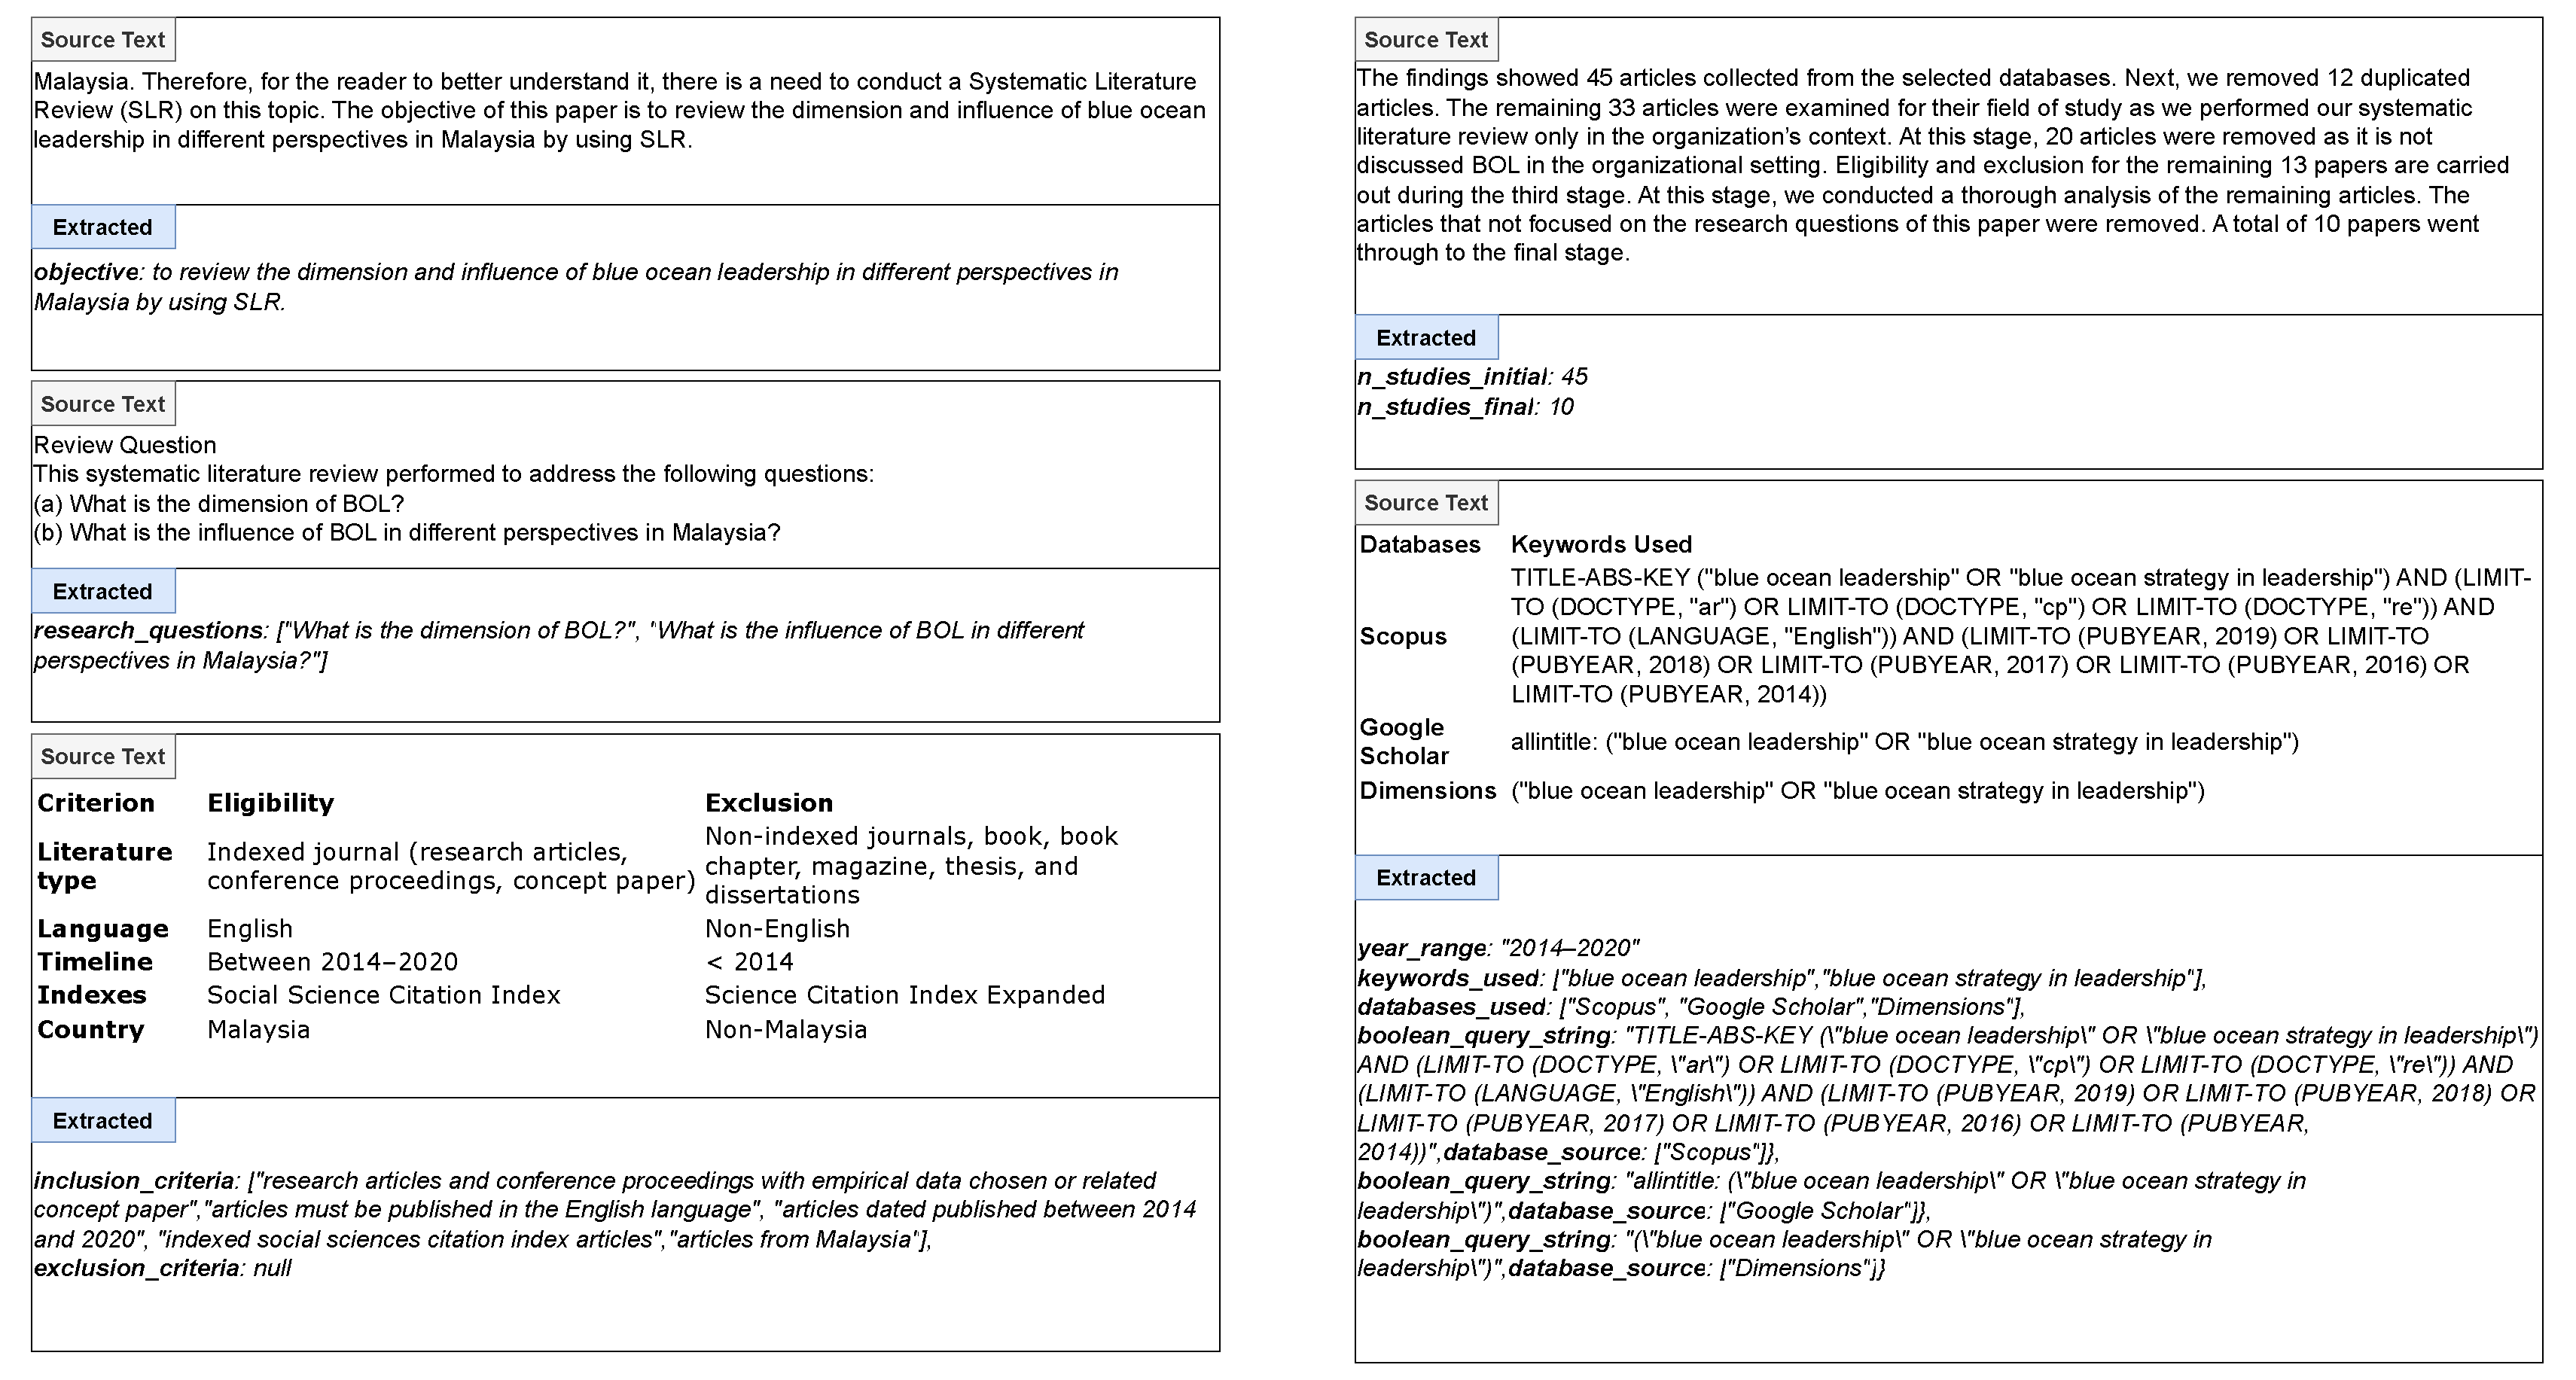
\includegraphics[width=\linewidth]{figures/example_2.pdf}
    \caption{Grounded extraction of review key information. Verbatim source spans from the PDF are transformed into structured schema fields via the verify-then-repair pipeline.}
    \label{fig:extraction_example}
\end{figure}

The final output is an evidence-centric structured representation integrating only verified extractions with OpenAlex metadata. For comparability, temporal search constraints are normalized to a canonical year-range format anchored to the publication year, while preserving original values. Table~\ref{tab:sysrev_field_coverage} summarizes metadata and methodological field coverage across the corpus after enrichment.

\begin{table}[t]
\centering
\sffamily
\renewcommand{\arraystretch}{1}
\caption{Availability of fields across \webisSRCorpus. Percentages use all 334,893 records as the denominator, except for the effectively usable subset, whose percentage uses the 107,611 records with extraction.}

\begin{tabular*}{\columnwidth}{@{\extracolsep{\fill}}lrr}
\toprule
\textbf{Subset} & \textbf{Count} & \textbf{Percentage} \\
\midrule
Total available sysrevs & 334,893 & 100\% \\
\midrule
\multicolumn{3}{l}{\textit{Availability of core materials}} \\
w/ title & 334,893 & 100.0\% \\
w/ abstract & 232,628 & 69.5\% \\
w/ extracted fields & 107,611 & 32.1\% \\
w/ all fields filled & 1,635 & 1.5\% of extracted \\
\midrule
\multicolumn{3}{l}{\textit{Review methodology fields}} \\
w/ objective & 100,203 & 29.9\% \\
w/ research questions & 17,686 & 5.3\% \\
w/ keywords used & 79,141 & 23.6\% \\
w/ boolean queries & 18,586 & 5.5\% \\
w/ inclusion criteria & 96,527 & 28.8\% \\
w/ exclusion criteria & 79,529 & 23.7\% \\
w/ date range & 334,891 & 100.0\% \\
\midrule
\multicolumn{3}{l}{\textit{Search, study-flow, and citation data}} \\
% PREVIOUSLY: \multicolumn{3}{l}{\textit{Search and study flow data}} \\
w/ databases & 98,980 & 29.6\% \\
w/ initial study count & 85,852 & 25.6\% \\
w/ final included-study count & 92,733 & 27.7\% \\
w/ resolved OpenAlex references & 334,893 & 100.0\% \\
% PREVIOUSLY:
% w/ paper counts retrieved & 85,852 & 25.6\% \\
% w/ paper counts included & 92,733 & 27.7\% \\
% w/ paper references included & 334,893 & 100.0\% \\
\midrule
\textbf{All essentials complete} & \textbf{78,058} & \textbf{72.5\% of extracted} \\
\bottomrule
\end{tabular*}
\label{tab:sysrev_field_coverage}
\end{table}


\subsection*{Query normalization}
\label{sec:query-norm}
Reported search strategies are expressed in heterogeneous, database-specific query languages, which prevents their direct execution in a single retrieval environment. To make them comparable and executable, each reported strategy is transformed into a simplified Boolean expression that can be issued to the OpenAlex API. The resulting normalized queries are included in the corpus as a separate field.

The normalization retains only topical terms and the fundamental logical operators \texttt{AND}, \texttt{OR}, and \texttt{NOT}. Database-specific syntax is removed, including explicit field tags (e.g.\ \texttt{TITLE-ABS-KEY} in Scopus or \texttt{[mesh]} in PubMed) and metadata constraints such as language or publication-type filters. Temporal restrictions are not embedded in the Boolean string; instead, the extracted year-range metadata is retained separately and can be applied externally at query time.

Normalization is performed using an instruction-tuned large language model (Qwen3-32B) applied to the reported Boolean queries or keyword lists. The model is prompted with a few-shot approach to preserve the topical vocabulary and high-level logical structure of each strategy without introducing concepts or search terms not present in the original formulation. Lightweight rule-based post-processing then ensures syntactic validity of the resulting Boolean expressions.

Some strategies cannot be normalized without additional assumptions. When numeric placeholders reference external term lists not provided in the review, or when the reported strategy contains insufficient information to construct a meaningful query, the normalized query is set to \texttt{null}. Likewise, when post-processing cannot produce a valid, non-empty Boolean expression, the query is set to \texttt{null}. Two query variants are produced where the source permits: normalized Boolean strategies reconstructed from reported search strings, and keyword-based queries constructed from reported keyword lists where a full Boolean query is unavailable.   % Methods
\section*{Data Records}
%%% https://www.nature.com/sdata/submission-guidelines
% - explain what the dataset contains, including the repository where the dataset is hosted, an overview of the data files and their formats, and any folder structure. 
% - Each external dataset should be cited using our data citation format. 
% - define any column headings, variable names, or other fields/metadata if you believe these would not be understood to users (e.g. terms like "gender" or "year" may not need explanation, but any bespoke terms may do). 
% - do not include summary statistics in this section, but see the description below if you wish to include these.

The \webisSRCorpus{} corpus is archived at Zenodo (\href{https://doi.org/10.5281/zenodo.18431942}{\texttt{10.5281/zenodo.18431942}}). The current release contains one JSON Lines file, \texttt{sr4all\_full.jsonl}. Each line corresponds to one JSON-encoded systematic review record, so the corpus can be processed sequentially without loading the full archive into memory. Full-text PDFs are not redistributed as part of the archive.

The released record type is the review record. Each record is anchored by the OpenAlex work identifier stored in \texttt{id}. Where available, the record also includes the work DOI in \texttt{doi}. These identifiers link the released records back to the underlying scholarly work and its citation context. Table~\ref{tab:data-record-reviews} provides a compact overview of the fields included in the released review records.

The review records combine three data layers within the same JSON object. First, a bibliographic metadata layer is available for all records. Second, a citation layer provides the resolved OpenAlex reference list and related citation counts. Third, records with accessible full texts and successful extraction contain an additional methodological layer derived from the extraction pipeline.

The bibliographic metadata layer and the citation layer are present for all 301,871~review records. The citation layer is attached directly to the same review-level identifier rather than stored in a separate file. As a result, users do not need to join multiple internal record types to reconstruct a review entry. The outgoing references listed for a review are represented by OpenAlex identifiers, which link the review to the cited works in the OpenAlex graph.

The methodological layer is available only for the subset of reviews with accessible full texts and successful verified extraction. This layer stores review aims, search-related information, eligibility criteria, study counts, and normalized temporal restrictions. These fields are attached to the same review record as the metadata and references, so the presence of extracted information can be checked directly within a single JSON object. Missing methodological values remain \texttt{null} or are omitted when no verified value could be retained.

\begin{table}[t]
\centering
\small
\sffamily
\renewcommand{\arraystretch}{1.15}
\caption{Data record overview for review records in \webisSRCorpus. \textit{Key(s)} denotes the top-level JSON keys in the released file, \textit{Description} summarizes their content, and \textit{Role} indicates how the fields support reuse.}
\label{tab:data-record-reviews}

\begin{tabular}{@{}p{1.9cm}p{4.4cm}p{6.1cm}p{2.0cm}@{}}
\toprule
\textbf{\textsf{Group}} & \textbf{\textsf{Key(s)}} & \textbf{\textsf{Description}} & \textbf{\textsf{Role}} \\
\midrule
Identifiers & \texttt{id}, \texttt{doi} & OpenAlex work identifier and DOI for the review record. & Primary linkage \\

Metadata & \texttt{title}, \texttt{abstract}, \texttt{year}, \texttt{type}, \texttt{source}, \texttt{language} & Core bibliographic metadata for each review. & Discovery and filtering \\

Subject labels & \texttt{field}, \texttt{subfield}, \texttt{topics}, \texttt{keywords} & OpenAlex field assignments and topical annotations. & Domain analysis \\

Authorship & \texttt{authors} & Author identifiers, names, and affiliation strings, where available. & Provenance \\

Citation context & \parbox[t]{4.4cm}{\texttt{cited\_by\_count}, \texttt{referenced\_works\_count}, \texttt{referenced\_works}, \texttt{references\_abstract\_}\\\texttt{coverage}} & Citation counts, resolved OpenAlex reference list, and summary information about abstract coverage among referenced works. & Retrieval and screening evaluation \\

Access & \texttt{pdf\_url} & Source PDF link when OpenAlex provides one. & Full-text access \\

Review aims & \texttt{objective}, \texttt{research\_questions} & Extracted statements of the review objective and explicit research questions. & Method analysis \\

Search strategy & \parbox[t]{4.4cm}{\texttt{keywords\_used}, \texttt{exact\_boolean\_queries}, \texttt{databases\_used}, \texttt{snowballing}} & Extracted search terms, normalized Boolean queries, named databases, and citation-chasing indicator. & Retrieval studies \\

Eligibility and flow & \parbox[t]{4.4cm}{\texttt{inclusion\_criteria}, \texttt{exclusion\_criteria}, \texttt{n\_studies\_initial}, \texttt{n\_studies\_final}} & Extracted eligibility criteria and study-count information from the review workflow. & Screening studies \\

Temporal scope & \parbox[t]{4.4cm}{\texttt{year\_range}, \texttt{year\_range\_normalized}, \\\texttt{year\_range\_normalization\_rule}} & Reported search-year restrictions, their normalized form, and the applied normalization rule. & Query reconstruction \\
\bottomrule
\end{tabular}

\end{table}

   % Data Records
\section*{Technical Validation}
%%% https://www.nature.com/sdata/submission-guidelines
% - describe the experiments, analyses or checks needed to support the technical quality of the dataset, with any supporting figures and tables, as needed.

The automated extraction pipeline includes two internal verification stages, evidence-span alignment and LLM-based factual verification, that discard unsupported extractions before inclusion in the final corpus (see Methods). To assess the quality of the extracted fields independently of these automated checks, we conduct a manual expert validation on a stratified sample of the corpus.

\subsection*{Sampling design}
The validation population comprises the 72,678 reviews with parsed full texts, i.e.\ all documents on which the extraction pipeline was executed. The unit of validation is the document: for each sampled review, all extracted methodological fields are assessed against the source PDF. Results are reported per field type.

The sample size is determined using the standard formula for estimating a proportion~\cite{cochran:1977}. At a 95\% confidence level ($z = 1.96$) and a margin of error of $\pm 5$ percentage points ($e = 0.05$), and using the conservative assumption $p = 0.5$, which maximizes the required sample size independently of the true extraction quality, the base sample size is
\[
n_0 = \frac{z^2 \, p(1-p)}{e^2} = \frac{1.96^2 \times 0.5 \times 0.5}{0.05^2} \approx 385.
\]
Applying the finite population correction for $N = 72{,}678$,
\[
n = \frac{n_0}{1 + \frac{n_0 - 1}{N}} \approx 383,
\]
which we round up to 385 documents. Because the correction is negligible at this population size, the sample size is effectively independent of $N$.

Documents are drawn by proportionate stratified random sampling, with strata defined by field and by document length. Stratification ensures that non-medical disciplines and longer documents, where parsing and extraction are expected to be more difficult, are represented according to their share of the population.

As not every review reports every methodological field, per-field sample sizes vary with field coverage: frequently reported fields (e.g.\ objective, date range) occur in most sampled documents, while sparsely reported fields (e.g.\ databases queried, research questions) occur in fewer. Estimates for sparsely covered fields are correspondingly less precise. We therefore report the exact number of judgments and the associated confidence interval for each field.

\subsection*{Annotation protocol}
Three annotators with expertise in systematic review methodology assess the sample against written annotation guidelines, fixed before annotation, that define correct and incorrect extractions and specify the treatment of boundary cases such as partial extractions and formatting variants. A shared subset of 80 documents is annotated independently by all three annotators to quantify inter-annotator agreement; the remaining 305 documents are divided evenly among them.

For each sampled document, two complementary assessments are performed. First, every non-null extracted field is compared against its verbatim evidence span and the source PDF, yielding a per-field correctness judgment (precision). Second, every field for which the pipeline returned no value is checked against the source PDF to determine whether the corresponding information is in fact reported, yielding an estimate of coverage (recall). The latter quantifies the pipeline's stated trade-off of completeness for precision.

Inter-annotator agreement on the shared subset is measured with Fleiss'~$\kappa$~\cite{fleiss:1971}; disagreements are resolved by discussion, and the adjudicated labels are used for the final estimates.

\subsection*{Reported estimates}
For each field type, precision and recall are reported together with 95\% Wilson score intervals~\cite{wilson:1927}, which remain accurate for proportions close to the boundaries~\cite{brown:2001}, the regime expected for a precision-oriented pipeline. Systematic error patterns observed during annotation are summarized in a qualitative error analysis.

% TODO 
% Sampling design (report the concrete sample composition)
% Annotation protocol
% Inter-annotator agreement
% Results Table
% Error analysis
   % Technical Validation
\section*{Usage Notes}
%%% https://www.nature.com/sdata/submission-guidelines
% - OPTIONAL SECTION
% - can be used to provide information that may assist other researchers who reuse your data. 
% - Most commonly these are additional technical notes about how to access or process the data.
% - do not use this section to write a conclusions section, general selling points, worked cases studies, or similar, as we do not publish these. 

The \texttt{referenced\_works} field contains the outgoing references associated with each systematic review in OpenAlex. These references should not be interpreted as the set of studies ultimately included in the review, as bibliographies may also contain methodological literature, background sources, previous reviews, and other cited works. The field can nevertheless serve as a reproducible cited-work target for retrieval experiments or weak supervision. Accordingly, evaluation against \texttt{referenced\_works} should be interpreted as recovery of cited works rather than recovery of included studies, and not as conventional systematic-review screening performance.
   % Usage Notes (optional)
\section*{Data Availability}
%%% https://www.nature.com/sdata/submission-guidelines
% - describe what data is being shared, and where to find it, is the “Data Record” section. Please ensure this section is detailed enough to allow reader to find and use your dataset.
% - we require a short “Data Availability” statement to repeat the main points in the Data Record, meaning some duplication is expected. We suggest repeating the lists of accession numbers, URLs, and the reference numbers for all datasets associated with the paper.
% - We request the additional statement as Data Availability statements (DASs) are a key publication standard. They are present in many other research articles, so we require them to align with wider practice and ensure readers who use them can find information quickly and easily. In addition, some indexing and scraping efforts may look in the DAS discern which datasets are linked to our articles, so the extra heading and information can be additionally helpful.

\webisSRCorpus{} is available from Zenodo at \href{https://doi.org/10.5281/zenodo.18431942}{\texttt{10.5281/zenodo.18431942}}. The current release contains the file \texttt{sr4all\_full.jsonl}, which stores 301,871 systematic review records in JSON Lines format. Full-text PDFs are not redistributed as part of the archive; where available, source access links are retained in the \texttt{pdf\_url} field.
   % Data Availability + Code Availability
\section*{Code Availability}
%%% https://www.nature.com/sdata/submission-guidelines
% - a statement indicating whether and how and custom code can be accessed, including any restrictions to access. 
% - can also include information on the versions of any software used, if relevant, and any specific variables or parameters used to generate, test, or process the current dataset if these are not included in the Methods.
% - see our policy on code availability for more information. 
% - The code availability statement should be placed at the end of the manuscript, immediately before the references. 
% - If no custom code has been used then the statement is still required in order to state this. 

   % Author Contributions / Competing Interests / Funding / Acknowledgements

\bibliographystyle{unsrtnat}    % numbered by order of appearance
\bibliography{scidata--sr4all-lit}

\end{document}
